%!TEX root = ../../thesis.tex

\chapter{Introduction and theoretical motivation}
\label{chap:motivation}
%!TEX root = ../../thesis.tex

The Standard Model (SM) of particle physics is the theory of sub-atomic particles.
It is the culmination of many decades of progress in both experimental and theoretical
quantum physics during the 20th century. It has enjoyed unparalleled success in describing 
a wide range of phenomena, which have been experimentally verified to an extraordinary 
degree of precision.

A crucial aspect of the SM is the generation of non-zero particle masses, which are 
forbidden by underlying symmetries of the theory but remain an experimental fact. 
They are generated by 
the Higgs mechanism of electroweak symmetry breaking, which also predicts the existence of 
a massive scalar particle, the Higgs boson, whose mass is a free parameter of the theory. 
As the only undiscovered particle of the SM, the discovery of the Higgs boson was 
a primary goal of the LHC physics program, which began in 2010.

A brief introduction to the SM is given in \Section~\ref{sec:sm}, outlining the 
particle content and interactions of the theory. In \Section~\ref{sec:ewsb}, electroweak 
symmetry breaking is described in detail. Then, some properties of the Higgs boson are 
described in \Section~\ref{sec:properties}, and the constraints upon its mass prior to the 
LHC are detailed in \Section~\ref{sec:prior_constraints}.

\section{The Standard Model of particle physics}
	\label{sec:sm}
	%!TEX root = ../../thesis.tex

The Standard Model of particle physics (SM) is a quantum field theory describing
the kinematics and interactions of sub-atomic particles. The dynamics of such a 
theory are determined by the symmetries respected by the Lagrangian density.
The SM is invariant under local transformations of the \SMgroup gauge group,
resulting in the strong, weak and electromagnetic forces of nature and determining
the particle content of the theory. Additionally, invariance under global 
transformations of the Poincaré group ensures the theory is identical in all 
inertial frames of reference, as asserted by special relativity.

Each gauge theory of the SM describes the dynamics of a force of nature, which 
is mediated by a number of gauge bosons and couples to a conserved current, in 
accordance with Noether's theorem. Quantum chromodynamics (QCD) describes the strong 
interaction, is mediated by eight gluons and couples to colour charge. Quantum 
electrodynamics (QED) describes the electromagnetic interaction, is mediated by the 
photon and couples to electric charge. The weak interaction is mediated by the massive 
\PWpm and \PZzero bosons and is understood within the context of electroweak theory (EW),
a unification of the electromagnetic and weak interactions. A quantum field theory of
gravity is not included in the SM. It is important to note that the gauge groups of the
strong and weak interactions are non-abelian. Physically, this means that the
gauge bosons are themselves charged and therefore experience self-interactions.

\begin{figure}
	\includegraphics[width=\largefigwidth]{tex/motivation/sm_particles}
	\caption{The particle content of the Standard Model. Mass data from \cite{PDG}.}
	\label{fig:sm_particles}
\end{figure}

The elementary particles of the SM are summarised in \Figure~\ref{fig:sm_particles}.
They are naturally separated into bosons (integer spin) and fermions (half-integer spin).
In addition to the gauge bosons previously introduced, the Higgs boson is a by-product
of electroweak symmetry breaking (described in \Section~\ref{sec:ewsb}) and its
couplings are proportional to mass. The fermions are categorised according to the
interactions they experience, or equivalently the charges they posses: quarks
(strong, electromagnetic, weak), charged leptons (electromagnetic, weak) and neutrinos 
(weak). Most particles also have an associated antiparticle with identical mass
but inverted internal quantum numbers.

\section{Electroweak unification}
	\label{sec:ewsb}
	%!TEX root = ../../thesis.tex

The first theory of weak interactions was a four-point interaction with Fermi coupling 
constant \unit{$G_F = 1.166\times 10^{-5}$}{\GeV\rpsquared}. Although successful in 
describing low energy phenomena, such as nuclear $\beta$-decay and muon decay, at 
energies above \unit{\about300}{\GeV} the theory predicted cross sections which violate 
unitarity \cite{Aitchison}.

The solution was to introduce charged vector bosons (\PWpm bosons) to mediate the weak 
interaction, similar to the exchange of photons in \ac{QED}. However, unlike \ac{QED}, 
the weak interaction is short ranged and therefore its exchange bosons must be massive. 
Since the propagator for a particle of mass $m$ and momentum $p$ contains 
$1 / (p^2 - m^2)$, in the low energy limit we can relate to Fermi's theory and identify
\begin{equation}
	G_F \sim g^2 / m_{\PW}^2
\end{equation}
where $g$ is the coupling of the vector boson. Thus, at low energies, the strength of the weak interaction is suppressed by the mass of the exchange boson.

At this time, there were two key obstacles to unifying the electromagnetic and weak 
interactions. Firstly, the discovery of parity violation in cobalt-60 $\beta$-decay 
implied the weak interaction has a \VminusA structure, whereas \ac{QED} has a pure V 
structure \cite{Wu:1957}.\footnote{
	Five bilinear covariants can be constructed from the Dirac $\gamma$ matrices, which 
	are named according to how they transform under parity: scalar, pseudoscalar, vector, 
	axial vector and tensor.
}
Secondly, the \PWpm bosons are massive whilst photons are massless. This was a major problem because gauge bosons are inherently massless.\footnote{
	Consider the gauge transformation of a Yang-Mills gauge field 
	$\bvec{W}_{\mu} \rightarrow \bvec{W}_{\mu} - \partial_{\mu} \bvec{\alpha}(x)
	- g \lbrack \bvec{\alpha}(x) \times \bvec{W}_{\mu} \rbrack$. Clearly the mass term 
	$-\tfrac{1}{2}m^2 \bvec{W}_{\mu} \cdot \bvec{W}^{\mu}$ is not gauge invariant, and 
	hence the gauge boson is massless.}
In fact, fermion masses were also forbidden by the chiral nature of the weak interaction, 
but were known to exist.\footnote{
	Consider a spinor as the sum of its left- and right-handed chiral states 
	$\psi = \psi_L + \psi_R$. Then the Dirac mass term is $-m \bar{\psi} \psi = 
	-m (\bar{\psi}_R \psi_L + \bar{\psi}_L \psi_R)$. For a chiral theory, $\psi_L$ and
	$\psi_R$ behave differently under gauge transformations and thus the mass term is not gauge invariant.
}

Glashow's proposal of an \EWgroup group was a major step forward \cite{Glashow:1961}. 
This model describes three gauge fields \rowthreevec{W^1_{\mu}}{W^2_{\mu}}{W^3_{\mu}} 
which couple to weak isospin $T$ with strength $g$, and a single gauge field $B_{\mu}$ 
which couples to weak hypercharge $Y$ with strength $g'$. The subscript $L$ indicates 
that only left-handed chiral particles couple to the $W^i_{\mu}$ fields, explaining the 
\VminusA nature of the weak interaction whilst preserving \ac{QED}. The physical gauge 
fields are obtained through the mixing of these fields
\begin{align}
	W^{\pm}_{\mu} &= (W^1_{\mu} \mp i W^2_{\mu}) / \sqrt{2} \label{eq:Wfield} \\
	Z_{\mu} &= \cos\theta_W W^3_{\mu} - \sin\theta_W B_{\mu} \label{eq:Zfield} \\
	A_{\mu} &= \sin\theta_W W^3_{\mu} + \cos\theta_W B_{\mu} \label{eq:Afield}
\end{align}
where
\begin{align}
	\cos\theta_W = g/\sqrt{g^2 + g'^2} && \sin\theta_W = g'/\sqrt{g^2 + g'^2} \,. \label{eq:weak_mixing}
\end{align}
We identify $W^{\pm}_{\mu}$ with the \PWpm bosons, $A_{\mu}$ with the photon 
and $Z_{\mu}$ with a new neutral \PZ boson. Weak neutral currents were later confirmed 
experimentally \cite{Gargamelle:1973}. 

Glashow's \EWgroup theory therefore predicts the interaction of fermions, in left-handed 
\SUgroup{2} doublets and right-handed \SUgroup{2} singlets (see 
\Table~\ref{tab:ew_fermions}), with \PWpm, \PZ and \Pphoton 
exchange bosons. Gauge boson self-interactions are also expected due to the non-abelian 
nature of the \ac{EW} theory. The \PWpm bosons couple to weak isospin $T$ with strength 
$g$, the \PZ boson couples vectorially to $c_V$ and axially to $c_A$ with strength 
$g/(2\cos\theta_W)$, and the photon couples to electric charge $Q$ with strength 
$e = g\sin\theta_W$, where
\begin{align}
	c_V &= T_3 - 2 Q \sin^2\theta_W \quad\quad c_A = T_3 \\
	Q   &= T_3 + \frac{Y}{2} \,.
\end{align}

\begin{table}[b]
	\begin{tabular}{ccc@{\hskip 1cm}cccc}
		& & & $T$ & $T_3$ & $Y$ & $Q$ \\
		\hline
		\multirow{2}{*}{$\colvector{\Pnue\\ \Pe}_{\!\!\!L}$} & 
		\multirow{2}{*}{$\colvector{\Pnum\\ \Pmu}_{\!\!\!L}$} & 
		\multirow{2}{*}{$\colvector{\Pnut\\ \Ptau}_{\!\!\!L}$} & 
		$\tfrac{1}{2}$ & $+\tfrac{1}{2}$ & $-1$ & 0 \\
		& & & $\tfrac{1}{2}$ & $-\tfrac{1}{2}$ & $-1$ & $-1$ \\
		$\Pnue_R$ & $\Pnum_R$ & $\Pnut_R$ & 0 & 0 & 0 & 0 \\
		$\Pe_R$ & $\Pmu_R$ & $\Ptau_R$ & 0 & 0 & $-2$ & $-1$ \\
		\hline
		\multirow{2}{*}{$\colvector{\Pup\\ \Pdown'}_{\!\!\!L}$} & 
		\multirow{2}{*}{$\colvector{\Pcharm\\ \Pstrange'}_{\!\!\!L}$} & 
		\multirow{2}{*}{$\colvector{\Ptop\\ \Pbottom'}_{\!\!\!L}$} & 
		$\tfrac{1}{2}$ & $+\tfrac{1}{2}$ & $+\tfrac{1}{3}$ & $+\tfrac{2}{3}$ \\
		& & & $\tfrac{1}{2}$ & $-\tfrac{1}{2}$ & $+\tfrac{1}{3}$ & $-\tfrac{1}{3}$ \\
		$\Pup_R$ & $\Pcharm_R$ & $\Ptop_R$ & 0 & 0 & $+\tfrac{4}{3}$ & $+\tfrac{2}{3}$ \\
		$\Pdown'_R$ & $\Pstrange'_R$ & $\Pbottom'_R$ & 0 & 0 & $-\tfrac{2}{3}$ & $-\tfrac{1}{3}$ \\
	\end{tabular}
	\caption{The weak isospin $T$, weak hypercharge $Y$ and electric charge $Q$ quantum
	numbers assigned to the fermions. Right-handed neutrinos are decoupled from the 
	electroweak interaction, and were not originally included in the \ac{SM}. However, 
	recent observations of neutrino oscillations suggest these might exist.}
	\label{tab:ew_fermions}
\end{table}

Unfortunately, it was necessary to explicitly break the symmetry by adding mass terms for 
the \PWpm and \PZ bosons by hand. Initial attempts to invoke a mechanism of \ac{SSB} were 
hindered by the Goldstone theorem.



\subsection{The Goldstone theorem}
\label{sec:ewsb:goldstone}
\ac{SSB} arises when the vacuum state does not respect the symmetry in question. This can 
occur when a field acquires a non-zero vacuum expectation value. To see this, consider a 
complex scalar field $\phi$ described by the Lagrangian
\begin{equation}
	\mathcal{L} 
	= \parenths{\partial_{\mu}\phi^{\dagger}} \parenths{\partial^{\mu}\phi} 
	+ \mu^2 \phi^{\dagger}\phi - \lambda \parenths{\phi^{\dagger}\phi}^2
	\label{eq:lagr:goldstone}
\end{equation}
with positive $\mu^2$ and $\lambda$, giving a sombrero potential 
(\Figure~\ref{fig:sombrero}). 
Although $\mathcal{L}$ is invariant under global \Ugroup{1} transformations 
$\phi \rightarrow \eexp{-i\alpha} \phi$, there are infinite degenerate vacua
$\phi = \mu\eexp{-i\theta}/\sqrt{2\lambda}$ that are not invariant. In order to interact 
with the system, a single vacuum must be arbitrarily chosen, spontaneously breaking the 
\Ugroup{1} symmetry.

\begin{figure}[b]
	\includegraphics[width=\mediumfigwidth]{tex/motivation/sombrero}
	\caption{The sombrero potential, in which a vacuum state must be arbitrarily chosen, 
	spontaneously breaking the symmetry of the underlying Lagrangian.
	Fluctuations in the azimuthal direction correspond to a massless Nambu-Goldstone 
	boson. Fluctuations in the radial direction correspond to a massive Higgs boson.}
	\label{fig:sombrero}
\end{figure}

The Goldstone theorem states that \ac{SSB} of a continuous global symmetry will lead to 
the existence of a number of massless scalar Nambu-Goldstone bosons \cite{Goldstone:1962}.
This can be seen by considering radial and azimuthal excitations, $h\parenths{x}$ and 
$\theta\parenths{x}$, about the vacuum 
\begin{equation}
	\phi\parenths{x} = \frac{1}{\sqrt{2}} \sqbracs{v + h\parenths{x}} \eexp{-i\theta\parenths{x} / v}
\end{equation}
where $v = \mu/\sqrt{\lambda}$. When substituted into (\ref{eq:lagr:goldstone}), we get
\begin{equation}
	\mathcal{L} = \tfrac{1}{2}\partial_{\mu}\theta \partial^{\mu}\theta
	+ \tfrac{1}{2}\partial_{\mu}h \partial^{\mu}h
	- \mu^2 h^2
	+ \dots
\end{equation}
where the dots denote terms neither kinetic nor mass. 
We identify a massless Nambu-Goldstone boson (the $\theta$-mode) and a Higgs boson of 
mass $\sqrt{2}\mu$ (the $h$-mode).

In order to explain massive \PWpm and \PZ bosons, the electroweak symmetry must be broken.
But the Goldstone theorem suggested that this would predict massless scalar bosons, which
were not experimentally observed.



\subsection{The Higgs mechanism}
\label{sec:ewsb:higgs}
However, when \ac{SSB} of a continuous \textit{local} symmetry is studied, something 
remarkable happens. The Nambu-Goldstone bosons of the theory are `eaten' by the gauge 
bosons, giving them mass. The associated degrees of freedom appear as longitudinal 
components of the massive gauge bosons. This is known as the Higgs mechanism 
\cite{Englert:1964,Higgs:1964a,Higgs:1964b,Guralnik:1964,Higgs:1966}.

Consider the Lagrangian for a \Ugroup{1} gauge theory with a sombrero potential
\begin{equation}
	\mathcal{L} 
	= \parenths{D_{\mu}\phi}^{\dagger} \parenths{D^{\mu}\phi}
	- \tfrac{1}{4} F_{\mu\nu} F^{\mu\nu}
	+ \mu^2 \phi^{\dagger} \phi - \lambda \parenths{\phi^{\dagger} \phi}^2
	\label{eq:lagr:abelHiggs}
\end{equation}
where $D_{\mu} = \partial_{\mu} + iqA_{\mu}$ is the covariant derivative and $F_{\mu\nu} 
= \partial_{\mu}A_{\nu} - \partial_{\nu}A_{\mu}$ is the field tensor. This is invariant 
under local \Ugroup{1} transformations $\phi \rightarrow \eexp{-i\alpha\parenths{x}} \phi$
when accompanied by a gauge transformation of the potential 
$A_{\mu} \rightarrow A_{\mu} + \tfrac{1}{q}\partial_{\mu} \alpha\parenths{x}$.

We are free to choose the unitary gauge $\alpha\parenths{x} = -\theta\parenths{x}/v$,
altering the photon field $A_{\mu} \rightarrow A_{\mu} - \tfrac{1}{qv}\partial_{\mu} 
\theta\parenths{x}$ in the process. Ultimately, the final result is gauge-independent, 
but other choices make the gauge boson propagators gauge-dependent. Since the 
$\theta$-mode is `gauged away', excitations about the vacuum become
\begin{equation}
	\phi\parenths{x} = \frac{1}{\sqrt{2}} \sqbracs{v + h\parenths{x}}
\end{equation}
and the Lagrangian (\ref{eq:lagr:abelHiggs}) becomes
\begin{equation}
	\mathcal{L}
	= \frac{1}{2} q^2 v^2 A_{\mu} A^{\mu}
	- F_{\mu\nu}F^{\mu\nu}
	+ \frac{1}{2} \partial_{\mu}h \partial^{\mu}h
	- \mu^2 h^2
	+ \dots
\end{equation}
where the dots denote terms neither kinetic nor mass. 
The Nambu-Goldstone boson is no longer present and the photon has acquired a mass $qv$.
Again, there is a massive scalar Higgs boson as a by-product of the \ac{SSB}.



\subsection{Glashow-Salam-Weinberg electroweak theory}
The Higgs mechanism can be extended to non-abelian gauge theories, as was necessary to 
describe electroweak symmetry breaking \cite{Kibble:1967,Weinberg:1967,Salam:1968}.
Consider the Lagrangian for an \SUgroup{2}\cross\Ugroup{1} gauge theory with a sombrero
potential
\begin{equation}
	\mathcal{L} 
	= \parenths{D_{\mu}\phi}^{\dagger} \parenths{D^{\mu}\phi}
	- \tfrac{1}{4} \bvec{F}_{\mu\nu} \cdot \bvec{F}^{\mu\nu}
	- \tfrac{1}{4} G_{\mu\nu} G^{\mu\nu}
	+ \mu^2 \phi^{\dagger} \phi - \lambda \parenths{\phi^{\dagger} \phi}^2
	\label{eq:lagr:ewHiggs}
\end{equation}
where $D_{\mu} = \partial_{\mu} + \tfrac{i}{2} g \bvec{\tau} \cdot \bvec{W}_{\mu} + 
\tfrac{i}{2} g' Y B_{\mu}$ is the covariant derivative, and $\bvec{F}_{\mu\nu} = 
\partial_{\mu}\bvec{W}_{\nu} - \partial_{\nu}\bvec{W}_{\mu} - g \bvec{W}_{\mu} \cross 
\bvec{W}_{\nu}$ and $G_{\mu\nu} = \partial_{\mu}B_{\nu} - \partial_{\nu}B_{\mu}$ are the
field tensors. In this case, $\phi$ is an \SUgroup{2} doublet of complex scalar fields
\begin{equation}
	\phi = \colvector{\phi^+\\\phi^0} = \colvector{\frac{1}{\sqrt{2}} \parenths{\phi_1 + i\phi_2}\\ \frac{1}{\sqrt{2}} \parenths{\phi_3 + i\phi_4}}.
\end{equation}

Again, there are infinite degenerate vacua satisfying 
$\parenths{\phi_1^2 + \phi_2^2 + \phi_3^2 + \phi_4^2} = \mu^2/\lambda$. In analogue with 
the abelian Higgs mechanism, the unitary gauge sets the vacuum expectation values of 
$\phi_1$, $\phi_2$ and $\phi_4$ to be zero. Considering excitations about the vacuum
\begin{equation}
	\phi\parenths{x} = \colvector{0\\ \frac{1}{\sqrt{2}} 
	\sqbracs{v + h\parenths{x}}} \label{eq:higgs_doublet}
\end{equation}
the Lagrangian (\ref{eq:lagr:ewHiggs}) becomes
\begin{align}
	\mathcal{L} &= \tfrac{1}{8} g^2 v^2 \bvec{W}_{\mu} \cdot \bvec{W}^{\mu} - \tfrac{1}{4} \bvec{F}_{\mu\nu} \cdot \bvec{F}^{\mu\nu} + \tfrac{1}{8} v^2 g'^2 B_{\mu} B^{\mu} - \tfrac{1}{4} v^2 gg' B_{\mu} W_{3}^{\mu} - \tfrac{1}{4} G_{\mu\nu} G^{\mu\nu} \nonumber \\
	&\quad\quad {} + \tfrac{1}{2} \partial_{\mu}h \partial^{\mu}h - \mu^2 h^2 + \dots \\
	&= \tfrac{1}{4} g^2 v^2 W^{+}_{\mu} W^{-\mu} - \tfrac{1}{2} \parenths{\partial_{\mu}W^{+}_{\nu} - \partial_{\nu}W^{+}_{\mu}} \parenths{\partial^{\mu}W^{-\nu} - \partial^{\nu}W^{-\mu}} \nonumber \\
	&\quad\quad {} + \tfrac{1}{8} v^2 \parenths{g^2 + g'^2} Z_{\mu} Z^{\mu} - \tfrac{1}{4} \parenths{\partial_{\mu}Z_{\nu} - \partial_{\nu}Z_{\mu}} \parenths{\partial^{\mu}Z^{\nu} - \partial^{\nu}Z^{\mu}} - \tfrac{1}{4} F_{\mu\nu} F^{\mu\nu} \nonumber \\
	&\quad\quad {} + \tfrac{1}{2} \partial_{\mu}h \partial^{\mu}h - \mu^2 h^2 + \dots
\end{align}
where the dots denote terms neither kinetic nor mass, and the expression has been rewritten in terms of the physical gauge fields using (\ref{eq:Wfield}), (\ref{eq:Zfield})
and (\ref{eq:Afield}). The \PWpm bosons acquire a mass $gv/2$ and the \PZ boson acquires a
mass $v \sqrt{\parenths{g^2+g'^2}}/2$, while the photon is massless. Again, all Nambu-Goldstone bosons are gone and a Higgs boson has appeared as a by-product of the \ac{SSB}.

This theory predicts a striking relation between the gauge boson masses, using 
(\ref{eq:weak_mixing})
\begin{equation}
	m_{\PW} = m_{\PZ} \cos\theta_W
\end{equation}
which was experimentally verified once the \PW and \PZ bosons were discovered 
\cite{UA1:1989}. It also predicted a massive scalar Higgs boson, whose mass could not be 
determined from the other parameters of the theory.

Fermion masses can also be incorporated into \ac{EW} theory through Yukawa couplings.
Consider a coupling between the electron-type \SUgroup{2} doublet (see 
\Table~\ref{tab:ew_fermions}), the Higgs doublet $\phi$ given in 
(\ref{eq:higgs_doublet}), and the electron \SUgroup{2} singlet
\begin{align}
	\mathcal{L}_{\Pe}^{\text{Yuk}} &= -g_{\Pe} \parenths{\Plepton_{\Pe L} \phi \Pe_{R} + \Pe_{R} \phi^{\dagger} \Plepton_{\Pe L}} \\
	&= -\frac{g_{\Pe}}{\sqrt{2}} \sqbracs{v + h} \parenths{\Pe_{L} \Pe_{R} + \Pe_{R} \Pe_{L}}
\end{align}
where $g_e$ is the electron Yukawa coupling. The electron has acquired a mass 
$g_{\Pe}v/\sqrt{2}$ and the coupling of the Higgs boson to the electron is proportional 
to that mass.

Finally, we note a similar phenomenon in superconductors. There, the \Ugroup{1} symmetry 
of \ac{QED} is spontaneously broken, as in \Section~\ref{sec:ewsb:higgs}, giving mass to 
the photon and thereby producing the Meissner effect. In fact, Higgs bosons have been 
observed in the Raman spectra of superconductors \cite{Superconductivity}. However, a 
major difference is that the bosonic field is a Bose-Einstein condensate of loosely bound 
electron pairs (known as Cooper pairs), and therefore the \ac{SSB} is dynamic. This is 
only possible due to lattice vibrations of the underlying solid. It is natural to ask 
whether a similar dynamic mechanism could be used to break \ac{EW} symmetry, where the 
Higgs boson is a composite particle. This is an active area of theoretical research, 
though will not be explored here.

\section{Properties of the Higgs boson}
	\label{sec:properties}
	%!TEX root = ../../thesis.tex

The Higgs boson is predicted to have zero spin and positive parity, whilst being 
electrically neutral and colourless. It couples only to massive particles. Other 
properties, such as production cross sections and \acp{BR} of decay, must be calculated 
as a function of its mass, which is not predicted by the \ac{SM}.

% Experimental signatures for the Higgs boson are categorised according to production 
% mode and decay channel.

At a hadron collider such as the \acs{LHC}, the important production modes are \ac{ggF},
\ac{VBF}, Higgs-strahlung (\WH and \ZH) and top fusion (\ttH). Example Feynman diagrams 
are shown in \Figure~\ref{fig:feyn}. We note that the Higgs boson does not couple to 
massless gluons, therefore \ac{ggF} proceeds via loops of massive coloured particles 
(predominantly the top quark due to its large mass). 

\begin{figure}[b]
	\null\hfill
	\begin{subfigure}[b]{0.4\textwidth}
		\centering
		\includegraphics[width=\textwidth]{axodraw/ggF.pdf}
		\caption{Gluon-gluon fusion (ggF)}
		\label{fig:feyn:ggF}
	\end{subfigure}
	\hfill
	\begin{subfigure}[b]{0.4\textwidth}
		\centering
		\includegraphics[width=0.75\textwidth]{axodraw/VBF.pdf}
		\caption{Vector boson fusion (VBF)}
		\label{fig:feyn:VBF}
	\end{subfigure}
	\hfill\null
	\\\bigskip
	\null\hfill
	\begin{subfigure}[b]{0.4\textwidth}
		\centering
		\includegraphics[width=0.8\textwidth]{axodraw/VH.pdf}
		\caption{Higgs-strahlung (\WH and \ZH)}
		\label{fig:feyn:VH}
	\end{subfigure}
	\hfill
	\begin{subfigure}[b]{0.4\textwidth}
		\centering
		\includegraphics[width=0.625\textwidth]{axodraw/ttH.pdf}
		\caption{Top fusion (\ttH)}
		\label{fig:feyn:ttH}
	\end{subfigure}
	\hfill\null
	\caption{Examples of tree-level Feynman diagrams for the Higgs production processes relevant at the \ac{LHC}.}
	\label{fig:feyn}
\end{figure}

The production cross sections at the \acs{LHC} are shown in \Figure~\ref{fig:higgs_xs}. 
Whilst \ac{ggF} clearly dominates these rare processes, it suffers from large 
experimental backgrounds. The four other modes feature additional final state particles 
which can aid identification. For example, \ac{VBF} has two back-to-back quarks with no 
colour exchange between them.

\begin{figure}
	\includegraphics[width=0.48\textwidth]{tex/motivation/xs_lowrange}
	\hfill
	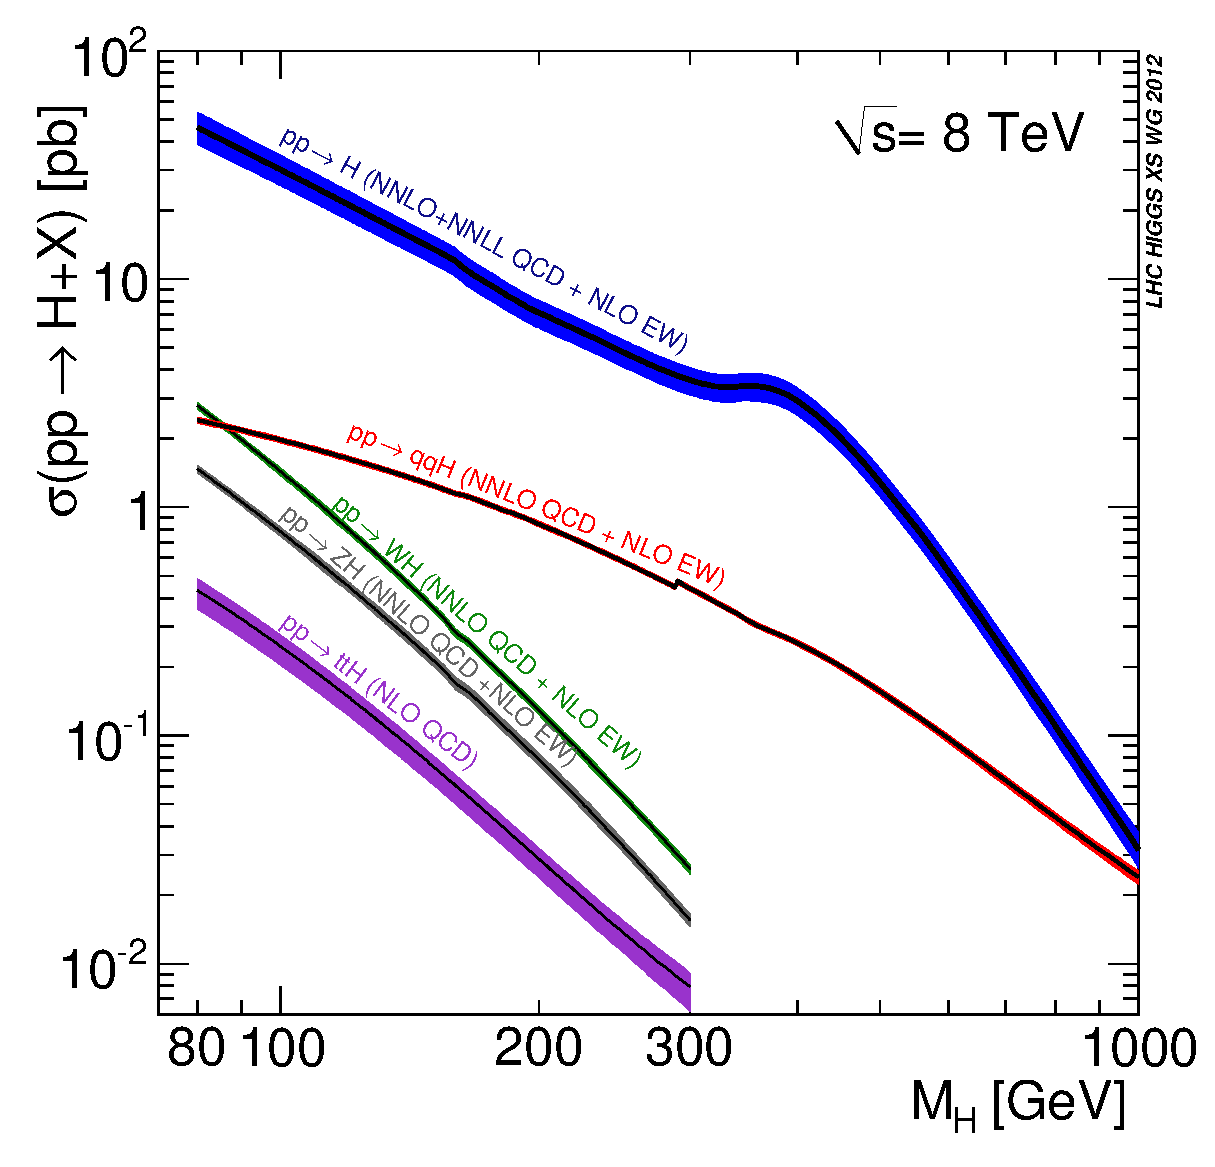
\includegraphics[width=0.48\textwidth]{tex/motivation/xs_fullrange}
	\caption{Higgs boson production cross sections versus mass at 
	\unit{$\sqrt{s} = 8$}{\TeV} for a low mass range (left) and an expanded mass range 
	(right) \cite{YR2}. Theoretical uncertainties are shown as bands. The production modes
	are \ac{ggF} (blue), \ac{VBF} (red), \WH (green), \ZH (grey) and \ttH (purple).}
	\label{fig:higgs_xs}
\end{figure}

Since the lifetime of the Higgs boson is very short, it is never directly observed in a 
detector. Therefore it is important to understand the \acp{BR} of its decays 
(\Figure~\ref{fig:higgs_br}). Na\"{i}vely, these are understood from the Higgs boson coupling to mass and the kinematic requirement $m_H > m_X + m_Y$ for a decay
\HepProcess{\PHiggs \HepTo XY}. This is complicated by off-shell particles (\eg a low mass
Higgs boson may decay to \HepProcess{\PW \PW^{*}}). 
Also, the \HepProcess{\Pphoton \Pphoton}, \HepProcess{\PZ \Pphoton} and 
\HepProcess{\Pgluon \Pgluon} decay modes are different since they feature massless 
particles, and therefore proceed via loops of massive charged particles (electric charge 
for \HepProcess{\Pphoton \Pphoton} and \HepProcess{\PZ \Pphoton}, colour charge for 
\HepProcess{\Pgluon \Pgluon}).

Designing a sensitive experimental search strategy for the Higgs boson can be difficult. 
In decay channels featuring weak bosons, the subsequent decay of the \PW or \PZ must also 
be considered. These are more likely to decay to quarks than leptons, but the former 
suffers from large backgrounds at hadron colliders. Similarly, the 
\HepProcess{\Pbottom \APbottom} has the largest \ac{BR} for low \mH but suffers from huge 
backgrounds. The sensitivity can be improved by combining with a more distinguished 
production mode, such as \WH or \ZH, but this reduces the production cross section.

\begin{figure}
	\includegraphics[width=0.48\textwidth]{tex/motivation/BR_lowrange}
	\hfill
	\includegraphics[width=0.48\textwidth]{tex/motivation/BR_fullrange}
	\caption{Branching ratios of Higgs boson decay versus mass for a low mass range (left) 
	and an expanded mass range (right) \cite{YR3}. Theoretical uncertainties are shown as 
	bands.}
	\label{fig:higgs_br}
\end{figure}

\section{Pre-LHC constraints on the Higgs boson mass}
	\label{sec:prior_constraints}
	%!TEX root = ../../thesis.tex

\subsection{Direct searches}

\subsection{Electroweak fits}

\bibliographystyle{thesis}
\bibliography{theory,pheno,mc,experiment}
